{
\renewcommand{\baselinestretch}{1.0}
\begin{figure}[t]
\begin{center}
\subfigure[Scaling a Hadoop sort benchmark up to 25 nodes.]{
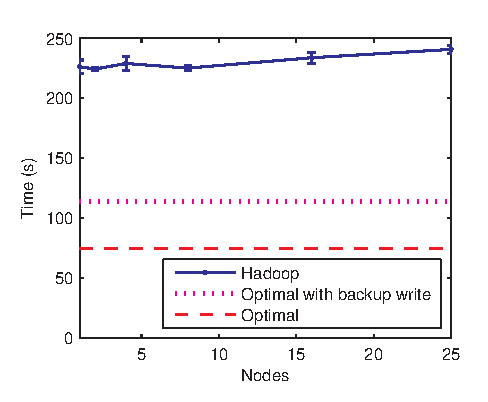
\includegraphics{fig_hadoop_sort.eps}
\label{fig:hadoopsort:scale}
}
\subfigure[Time breakdown into phases.]{
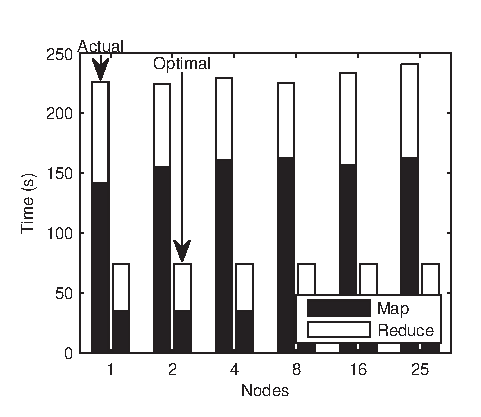
\includegraphics{fig_hadoop_breakdown.eps}
\label{fig:hadoopsort:breakdown}
}

\minicaption{Measured and optimal sort runtimes for a tuned Hadoop
  cluster.  Performance is about 3 times slower than optimal, and 2
  times slower than an optimal sort that includes an extra backup
  write for the map output, which is currently Hadoop's behavior}             
  {Hadoop scales well with 4~GB per node up to 25 nodes, but it is
  inefficient.  The measured runtime, optimal calculation, and optimal with
  backup write calculation are shown in {\bf (a)}.  The breakdown of
  runtime into map and reduce phases is shown in {\bf (b)}.

  % shows that a majority is spent in the map
  %, but there is considerable overhead
  %for creating and managing map and reduce tasks.  A breakdown
  %of the time in {\bf (b)} shows that a majority is spent in the map
  %phase, which includes time to setup the map and reduce tasks,
  %perform the map operation, and transfer data over the network to
  %the appropriate reducer. The reduce time includes the
  %actual sort and reduce operations, which will write the sorted data locally.}
}
\label{fig:hadoopsort}
\end{center}
\end{figure}
}

